\chapter{The Standard Model of Physics}\label{chap:SM}

\section{The History of Understanding the History of Everything}

In the beginning people knew nothing. What is the universe made of? Can you turn a rock into gold? What happens if you get smaller and smaller - is there a whole different world down there? These were just a small subset of questions our early ancestors would never know the answer to, since they all died out before the development of particle physics in the $20^{th}$ century. But let's entertain ourselves by examining a few of the early mental models they had, and how the persistent desire to improve these models led to the development of modern physics.

\subsection{The Basic Components}

It's somewhat strange at first glance that many ancient cultures had roughly the same classic elements, but upon examination of the things commonly found in nature, we can understand where these groupings came from. Most early building materials, food, and organic compounds came out of and into the earth. These things seemed to cycle endlessly and turn easily into each other, so the element of earth or clay logically served as a catch-all building block for all such materials. Chinese philosophy further divided wood and metal into their own categories separate from earth. Next came fire and water, distinct enough from earth to warrant separate categories of their own. Together, earth, water, and fire also roughly corresponded to the common states of matter (solid, liquid, gas/plasma), so it's understandable that these mental clusterings became common in many early philosophies. The elements of air and aether were somewhat unique to Greek thought however, and were probably later transported into India and folded into the classic Buddhist elements.

In all then, we had air, water, earth, fire, and aether in Greek philosophy, corresponding to the five Platonic solids~\cite{Plato}, and according to Empedocles~\cite{Empedocles}, bound together by love and strife. In Indian philosophy we had air, water, and earth, corresponding to different categories of food~\cite{Chandogya}. This evolved with Greek influence into the five elements of early Buddhism and Hinduism, each with their own associations~\cite{friesian}. In Chinese philosophy we had metal, wood, earth, water, and fire~\cite{Tao}. When combined with air and aether, the system was further expanded to form associations with the sun, moon, and five visible planets~\cite{friesian}.

And so we see how throughout the ancient world, a complex series of inter-related, "common-sense", and entirely wrong memetic systems came to dominate early philosophy. Based on pattern recognition and concept association rather than experimental evidence, these unscientific models guided intellectual pursuits for many centuries.

<The_Sceptical_Chymist>

<chemical revolution>

<John Dalton>

<Einstein brownian motion>

<Mendeleev>

\subsection{Elements Are Not Elemental}

\subsection{A New Subatomic World}

\section{Everything Is Particles}

\subsection{Electrifying Discoveries}

\subsection{Smashing the Proton}

\subsection{Photographing a Ghost}

\subsection{The Particle Nobody Ordered}

\subsection{A Confusing Explosion}

\subsection{Order to the Chaos}

\subsection{The Final Piece of the Puzzle}

\section{Physics Is Not Over}

\subsection{Problems with the Standard Model}

\subsection{What Particle Physicists Do All Day}

%%%%%%%%%%%%%%%%%%%%%%%%%%%%%%%%%%%%%%%%%%%%%%%%%%%%%%%%%%%

The purpose of the LHC and other similar colliders is to study physics at the most fundamental level of existence. We are interested in probing and measuring the smallest building blocks of nature, and in discovering how they go together. The most complete picture which we have to date is shown on the left side of Figure~\ref{SUSY}. In this model, known as the standard model, we describe the universe as a composition of leptons, quarks, and force carriers. Leptons include the well-known electron, as well as its nearly-invisible partner, the electron neutrino. Quarks include the building blocks of protons and neutrons, the up and down quarks. Furthermore, there are the heavier generations of these particles, which are just like the electron, electron neutrino, up quark, and down quark, only with more mass. We also have the force carriers (or gauge bosons) - photons for the electromagnetic force, gluons for the strong force, and W and Z bosons for the weak force. Finally, completing the picture is the recently-discovered Higgs boson, an excitation of the Higgs field which gives mass to the other fundamental particles. There are also the antimatter counterparts to these particles, which have opposite charge, though the neutral force carriers are their own antiparticles.

%\begin{figure}[t]
%    \centering
%    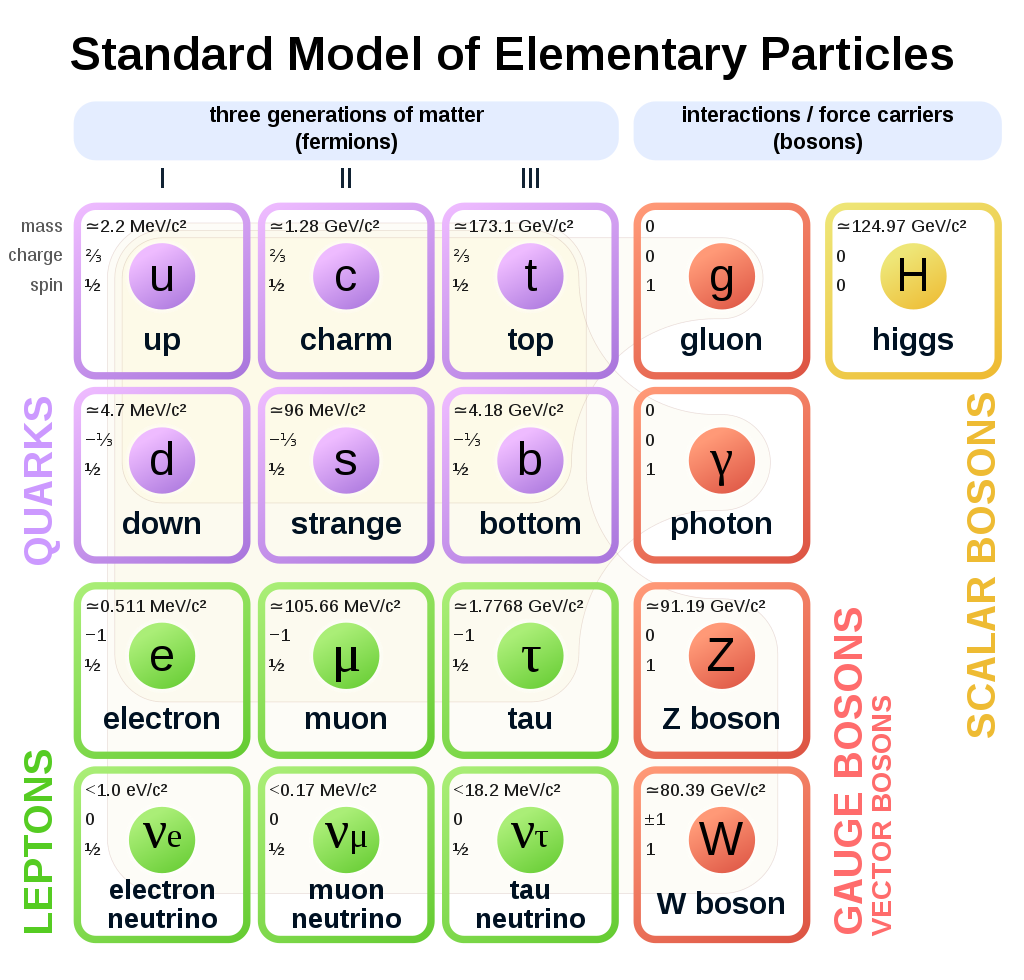
\includegraphics[width=0.7\linewidth]{images/standard_model.png}
%    \caption{The standard model.}
%    \label{standard_model}
%\end{figure}

\begin{figure}[t]
    \centering
    \includegraphics[width=0.7\linewidth]{images/SUSY.png}
    \caption{(left) The standard model. (right) Supersymmetric partners of standard-model particles. This diagram displays the squarks, sleptons, and gauginos which make up SUSY. The gauginos (from top to bottom, and left to right) are the gluino, photino, zino, the winos, and the Higgsinos. The photino, zino, and two neutral Higgsinos combine to form mass eigenstates $\tilde{\chi}^0_1, \tilde{\chi}^0_2, \tilde{\chi}^0_3, \tilde{\chi}^0_4$, which are called the neutralinos. The winos and two charged Higgsinos combine to form $\tilde{\chi}^\pm_1, \tilde{\chi}^\pm_2$, the charginos.}
    \label{SUSY}
\end{figure}

This model has produced some of the most accurate agreements between theory and experiment ever achieved in science, but we know that it does not describe the entire universe. For instance, the standard model only describes ordinary matter and antimatter, but these only account for about $5\%$ of the mass in the universe. Another $27\%$ is dark matter, and the remaining $68\%$ is dark energy. Gravity is not included in the standard model, as it remains the least-understood fundamental force. Many questions about it remain to be answered, such as why gravity is so much weaker than all the other forces. There is also the Higgs hierarchy problem, which relates to why the Higgs boson has the mass that it does \cite{hierarchy}. If we calculate the expected mass of the Higgs, we find that quantum loop corrections from virtual particles ought to push the mass up to an order of magnitude around the breakdown point of known physics, the Planck mass at $m_{Planck} = 10^{18}$ GeV. One way the Higgs can have a mass around 126 GeV is for bosonic and fermionic loop corrections to the Higgs mass (which have opposite sign) to cancel each other out.